\documentclass[14pt]{extarticle}
% math symbols
\usepackage{sfg}


\usepackage{amssymb,amsmath}
\synctex=1
% for different compilers
\usepackage{ifpdf}
% geometry of page
\usepackage[margin=2cm]{geometry}

% if pdflatex, then
\ifpdf
\usepackage[russian]{babel}
\usepackage[utf8]{inputenc}
\usepackage[unicode]{hyperref}
\usepackage[pdftex]{graphicx}
\usepackage{cmlgc}
% if xelatex, then
\else
% math fonts
\usepackage{fouriernc}
% xelatex specific packages
\usepackage[xetex]{hyperref}
\usepackage{xltxtra}	% \XeLaTeX macro
\usepackage{xunicode}	% some extra unicode support
\defaultfontfeatures{Mapping=tex-text}
\usepackage{polyglossia}	% instead of babel in xelatex
\usepackage{indentfirst}	% 
\setdefaultlanguage{russian}
% fonts
\newfontfamily\cyrillicfont{SchoolBookC}
\newfontfamily\cyrillicfontsf{TextBookC}
\setmonofont{Consolas}
\fi

% several pictures in one figure
\usepackage{subfig}
% calc in TeX expressions
\usepackage{calc}
% nice pictures and plots
\usepackage{pgfplots,tikz,circuitikz}
% different libraries for pictures
\usetikzlibrary{%
  arrows,%
  calc,%
  patterns,%
  decorations.pathreplacing,%
  decorations.pathmorphing,%
  decorations.markings,%
  intersections,%
  decorations.text%
}

\usepackage{tkz-euclide}

\usepackage{enumitem}
\renewcommand{\theenumi}{(\asbuk{enumi})}
\renewcommand{\labelenumi}{\asbuk{enumi})}
\AddEnumerateCounter{\Asbuk}{\@Asbuk}{\CYRM}
\AddEnumerateCounter{\asbuk}{\@asbuk}{\cyrm}

\begin{document}

\section*{Задача}

\subsection*{Условие}
Прямые $OA$, $OB$, $OC$ взаимно перпендикулярны. Проведена прямая $OX$. Установите зависимость между углами, которые $(OX)$ образует со своими проекциями на плоскости $AOB$, $BOC$, $AOC$.
\subsection*{Решение}
Пусть эти углы $\alpha_1$, $\alpha_2$ и $\alpha_3$. Узнаем проекции $OX$ на плоскости:
\begin{align*}
	OP_{AB}=OXcos{\alpha_1}; \\
	OP_{BC}=OXcos{\alpha_2}; \\
	OP_{AC}=OXcos{\alpha_3}.
\end{align*}
Из теорем Пифагора для плоскостей:
\begin{align*}
	OP_{AB}^2 = OP_A^2 + OP_B^2; \\
	OP_{BC}^2 = OP_B^2 + OP_C^2; \\
	OP_{AC}^2 = OP_A^2 + OP_C^2.
\end{align*}
Значит, $OP_{AB}^2+OP_{AB}^2+OP_{AB}^2 = 2(OP_A^2 + OP_B^2 + OP_C^2) = 
2OX^2$. Если сократить на $OX^2$, то получим
\begin{equation}
	cos{\alpha_1}^2 + 
	cos{\alpha_2}^2 + 
	cos{\alpha_3}^2 =
	2
\end{equation}
\newpage
\begin{figure}[h]
	\centering
	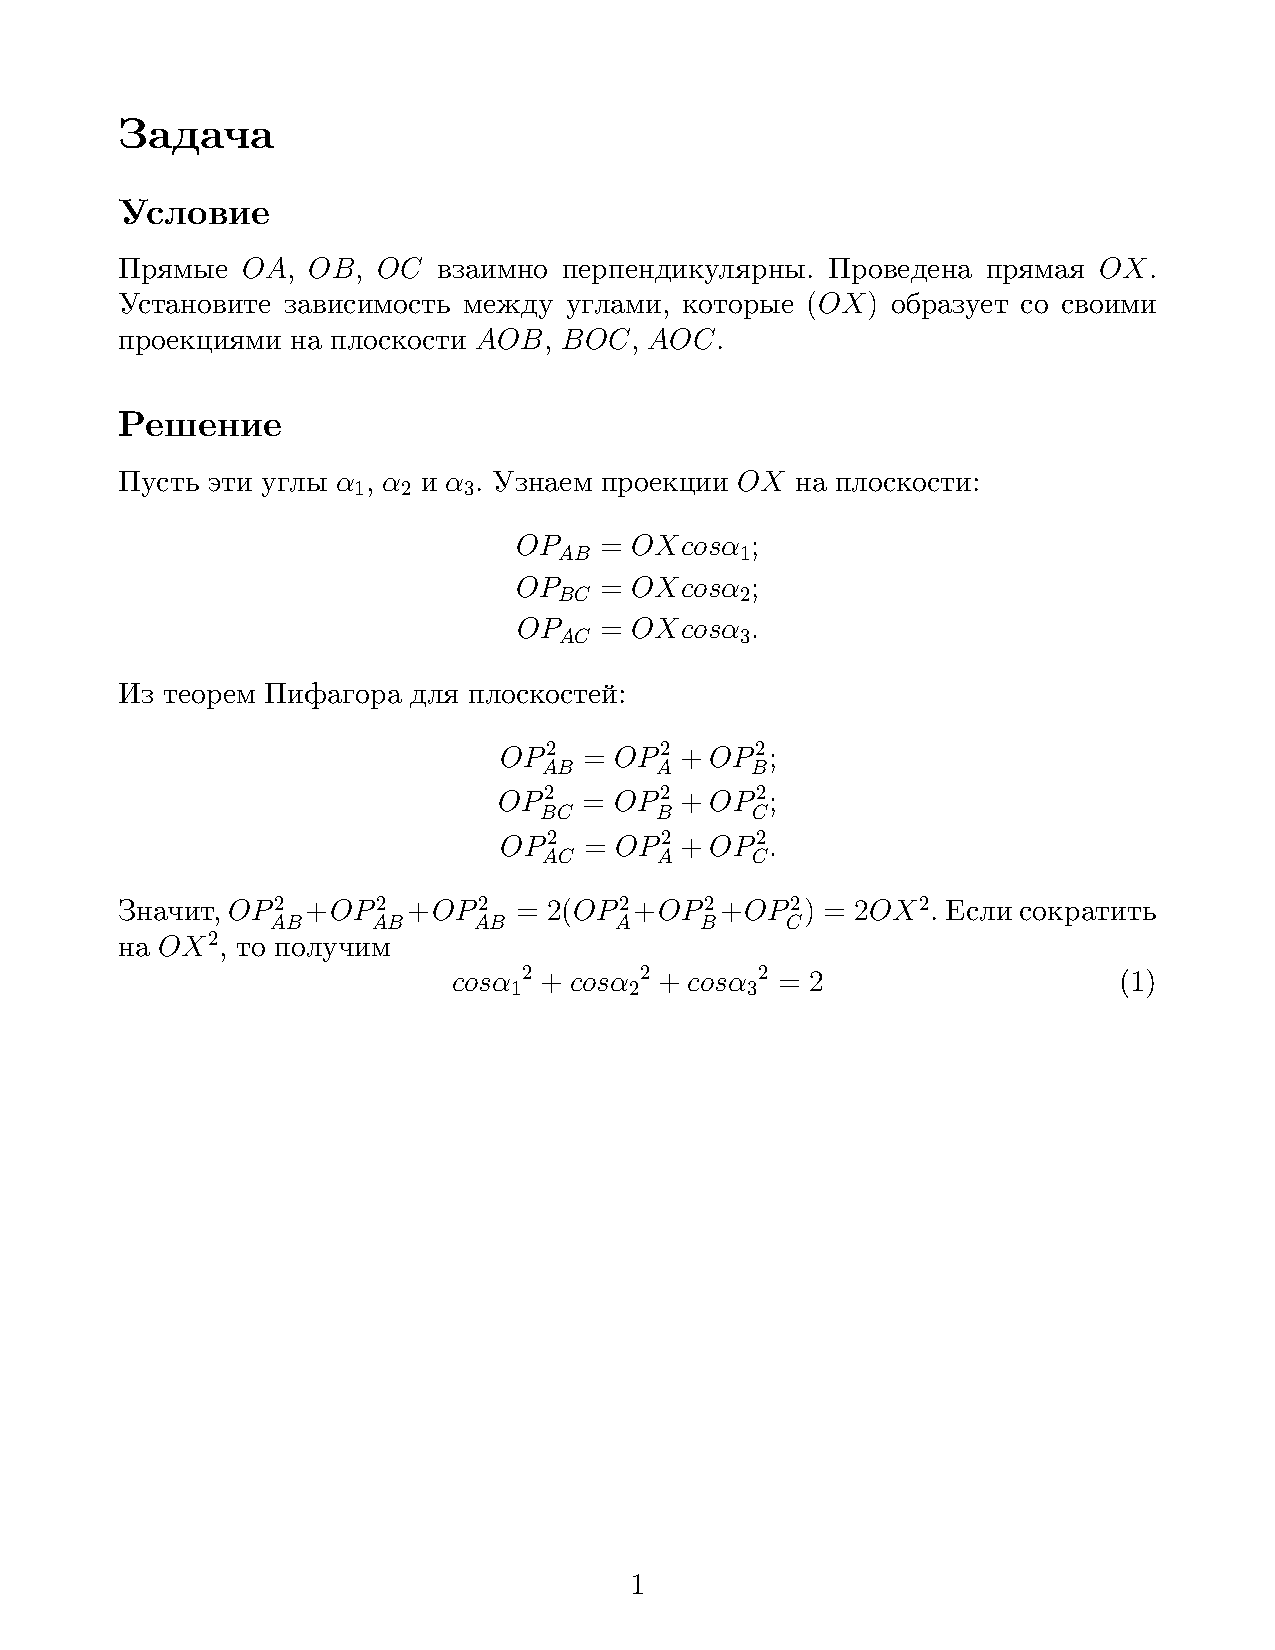
\includegraphics[width=1\textwidth]{{./13.2b}.png}
\end{figure}


\end{document}